\documentclass{article}\usepackage[]{graphicx}\usepackage[]{color}
%% maxwidth is the original width if it is less than linewidth
%% otherwise use linewidth (to make sure the graphics do not exceed the margin)
\makeatletter
\def\maxwidth{ %
  \ifdim\Gin@nat@width>\linewidth
    \linewidth
  \else
    \Gin@nat@width
  \fi
}
\makeatother

\definecolor{fgcolor}{rgb}{0.345, 0.345, 0.345}
\newcommand{\hlnum}[1]{\textcolor[rgb]{0.686,0.059,0.569}{#1}}%
\newcommand{\hlstr}[1]{\textcolor[rgb]{0.192,0.494,0.8}{#1}}%
\newcommand{\hlcom}[1]{\textcolor[rgb]{0.678,0.584,0.686}{\textit{#1}}}%
\newcommand{\hlopt}[1]{\textcolor[rgb]{0,0,0}{#1}}%
\newcommand{\hlstd}[1]{\textcolor[rgb]{0.345,0.345,0.345}{#1}}%
\newcommand{\hlkwa}[1]{\textcolor[rgb]{0.161,0.373,0.58}{\textbf{#1}}}%
\newcommand{\hlkwb}[1]{\textcolor[rgb]{0.69,0.353,0.396}{#1}}%
\newcommand{\hlkwc}[1]{\textcolor[rgb]{0.333,0.667,0.333}{#1}}%
\newcommand{\hlkwd}[1]{\textcolor[rgb]{0.737,0.353,0.396}{\textbf{#1}}}%
\let\hlipl\hlkwb

\usepackage{framed}
\makeatletter
\newenvironment{kframe}{%
 \def\at@end@of@kframe{}%
 \ifinner\ifhmode%
  \def\at@end@of@kframe{\end{minipage}}%
  \begin{minipage}{\columnwidth}%
 \fi\fi%
 \def\FrameCommand##1{\hskip\@totalleftmargin \hskip-\fboxsep
 \colorbox{shadecolor}{##1}\hskip-\fboxsep
     % There is no \\@totalrightmargin, so:
     \hskip-\linewidth \hskip-\@totalleftmargin \hskip\columnwidth}%
 \MakeFramed {\advance\hsize-\width
   \@totalleftmargin\z@ \linewidth\hsize
   \@setminipage}}%
 {\par\unskip\endMakeFramed%
 \at@end@of@kframe}
\makeatother

\definecolor{shadecolor}{rgb}{.97, .97, .97}
\definecolor{messagecolor}{rgb}{0, 0, 0}
\definecolor{warningcolor}{rgb}{1, 0, 1}
\definecolor{errorcolor}{rgb}{1, 0, 0}
\newenvironment{knitrout}{}{} % an empty environment to be redefined in TeX

\usepackage{alltt}
\usepackage{graphicx}
\usepackage{hyperref}
\title{SOP 85: Using NOAA Climate Records}
\author{Marc Los Huertos and Isaac Medina}
\IfFileExists{upquote.sty}{\usepackage{upquote}}{}
\begin{document}
\maketitle

\section{Introduction}
Raw data sets often come with untidy/non-useful formats or information that must first be cleaned or processed before an accurate and useful analysis of the contents can be done. After obtaining a data set there are some preliminary steps you must follow in order to get your data file into working order for your analysis. 

\subsection{Purpose}
This document is intended as a resource and guide to help you: 
\begin{itemize}
\item clone the climate narratives repository
\item upload your data file into the R environment using the Rstudio Server; and 
\item clean, organize and reformat the data to prepare it for analysis. 
\end{itemize}
Since this SOP (Standard Operating Procedure) is about uploading and cleaning your data file, it assumes you already know how to successfully login to Rstudio, connect to Marc's Github repositories and that you already downloaded a climate data file from the CDO website. If you haven't already done these steps, go back and download the following SOPs (linked here): 

\href{https://github.com/marclos/SOPs/raw/master/06_Rstudio_Github/Rstudio-and-Github_v03.pdf}{SOP 06: An Introduction to R, Rstudio, Github} 

\href{https://github.com/marclos/Climate_Change_Narratives/blob/master/Analysis_SOPs/SOP84_Obtaining_Climate_Records.pdf}{SOP: 84 Obtaining Climate Records}

\section{Connect to the Climate Narratives Repository}

In SOP 06 you did an excercise to connect to a test repository called ``Beginner's Luck''. This time we will connect to a new repository called ``Climate\_Change\_Narratives." You want to make sure that you \textbf{start a new project in R} connected to this repository since it will eventually house all the work you will do for the the climate project ``Do Weather Changes Matter?" 

\subsection{Start A New R Session}
We recommend starting a new R session for each project in order to have the most organized workspace. If when you sign into Rstudio it takes you directly to the active R session in which we were working on the ``Beginner's Luck Repository" follow these steps to create a new session

  \begin{itemize}
  \item If signed into an active session click on the red power button in the top right corner to ``Quit the current R session"
  \item Select Start New Session
  \end{itemize}

\subsection{Create A New Project linked to Climate\_Change\_Narratives}
To connect to the Climate Change Narratives Repository follow these steps:\\
\emph{Note: These steps are essentially the same as Step 5 in SOP 06 the difference being that we're linking to a different repository} \\

\begin{enumerate}
  \item In an an active Rstudio session click on \textbf{File}
  \item select \textbf{New Project} from the dropdown menu
  \item select \textbf{Version Control} and then select \textbf{Git}
  \item Get the new URL at \url{https://github.com/marclos/Climate_Change_Narratives}
  \item Click on the green button \textbf{Clone or Download} and ensure that the popup window says \textbf{CLONE WITH SSH}, if it says ``clone with HTTPS'' click on \textbf{Use SSH} 
  \item Copy the repository's URL 
  \item In Rstudio \textbf{Paste in the URL from Github}
  \item Under Project Directory Name type in ``Climate\_Change\_Narratives"
  \item Click on \textbf{Create Project} 
  \item Since were going to try to make changes to the repository this time, we'll need more access. \textbf{Send Marc an email} requesting to become a collaborator on the ``Climate\_Narratives\_Repository" and \textbf{accept the invitation} to become a collaborator on github
  \end{enumerate} 

\section{Preparing CSV file(s)}

\subsection{Upload CSV Files into Appropriate Rstudio Directory} 
The first step to getting your data into R is to upload it from your computer into the the Rstudio server online but to simplify our work in the future first \textbf{locate the file} in your computer and rename it using the following convention: \\ 
\begin{center}
\textbf{yourname\_region\_data}
\end{center}
where you fill in your firstname and a short descriptor for the region to which your data pertain. \\

Now follow these steps to upload the data into the Rstudio server:

  \begin{enumerate}
  \item In Rstudio click on the folder entitled \textbf{``Climate\_Change\_Narratives"} using the \textit{Files} tab in the lower right navigation GUI (Window 4 from SOP 06)
  \item Navigate to the folder entitled \textbf{``Data"} 
  \item Next click on the correct folder for your class, it should correspond to the term in which you are enrolled in the EA 30 class. For example: SP17 if you're enrolled in EA 30 spring semester of 2017.
  \item Use the upload button to select a file from your computer to upload into the rstudio server
  \begin{figure}[h]
  \includegraphics[scale=0.25]{"/home/CAMPUS/im022012/Climate_Change_Narratives/graphics/Upload_button"}
  \end{figure}
  \item In the popup window select \textbf{Browse} and navigate to the climate data file you downloaded from the CDO website (SOP 84). It should have the new name you gave it above (yourname\_region\_data)
  \item Click \textbf{Open} and then click \textbf{OK}. 
  
  \end{enumerate}

Your data file is now uploaded to the Rstudio server! All this means is that the actual file is in your workspace on the server. This however, doesn't mean that the file has been uploaded (or ``pushed") to the repository on Github.com. If Marc has added you as a collaborator already now would be a good time to go through the process of pulling, committing and pusing with Git. Ask Marc to guide you through this in lan, and continue to the next section. 


%\subsection{Preprocessing CSV files}

%In most cases, we don't need to preprocess the csv files before uploading them. However, Mac users have been confronted with a host of problems that has something to do with how Macs format CSV files. If you have any problems with reading or uploading your csv file on a Mac speak with the instructor or TA. \footnote{I will update this when I try using a Mac for this.}


\section{Reading CSV Files into R}

Now that we got the file saved onto the Rstudio Server it's time to tell R to read the file so we can look at the data! This will require telling R to read the file. In order to do this we will use R commands. (remember these commands are to be typed in the R ``console") %One way to confirm this is to look at the Rstudio tab \textbf{`Environment'} in the top right window, where the file shoud be listed. If you don't see anything here it's because the file has not yet been loaded into R. 

 \subsection{Finding the data path to the file}
In order to tell R to read the file you also have to let it know where the file is (R is funny that way). We use an R command to help us find the specific data path to the file. \\
In the console type in the following and then follow these steps: 
\begin{verbatim}
file.choose()
\end{verbatim}

\begin{itemize} 
\item press enter on your keyboard
\item in the resulting popup window navigate to the your saved data file and \textbf{double click} on it
\item Look at the console window.. under the command that you just typed you should now see a data path. The data path should look something like this: ``/home/CAMPUS/im022012/Climate\_Change\_Narratives/Data/test\_data/Singapore\_ClimateData.csv"  It is the location of where your file is saved on the server.
\item \textbf{Copy} the data path (including the parenthesis)
\end{itemize}

\subsection{Telling R to Read the Data File}

Now that we know where the data file is we will tell R to read it! In the console type in the following command and follow the next steps: 
\begin{verbatim}
read.csv()
\end{verbatim}

\begin{itemize}
\item This time before you press enter on the R command \textbf{Paste} in the data path you copied inbetween the parenthesis of the R command (be sure to include the parenthesis)
\item press enter
\item If your command worked you should see a bunch of text in your console window now. This means R read your file!
\end{itemize}

\subsection{Creating a Data Object}
So we made R read our file, however cool this might be, it is still not useful to us. In order to manipulate and do things with the data we need to tell R not only to read the file but also to store it in an object (such as a data frame) that we can manipulate. Follow these steps to tell R to read the file and store it in an object: \\

This time we will use the following R command\\
\begin{verbatim}
climate_data <- read.csv("the/file/path")
\end{verbatim}

\textbf{But be sure to use your actual data path!}

What this command is essentially doing is it's telling R to read the file and store it in an object called climate\_data ... if we really wanted to we could have actually named the object something else but climate\_data will suffice for now. \\ 

In R usually ``no news is good news" after you hit enter on a command. In other words, if you don't get red colored text describing an error, the program did something -- but now we need to figure out if it did something useful! Luckily there is a way to check if your command was successful in creating your object. All you have to do is check the \textbf{Environment} tab (in window 2). You should see your data object: climate\_data listed there. 



\section{Confirming the Proper Reading of the CSV file}


So we see that the data file is actually an object in R now. But what does it actually look like and what's in it? 
Since R was made to handle large data sets it tries not to overwhelm you with all the data at once but luckily the developers made a few commands to peak at the data to see if everthing is in order. We will try some of these commands now to look at few observations then we'll evaluate the structure of the dataframe and go on to finally plot the data!

\subsubsection{Viewing the 1st 6 Observations}
The following command allows you to view the first six observations of data in the data frame you created.
\begin{verbatim}
head(climate_data)
\end{verbatim}
Type it into the console and hit enter! You should get something that looks like the following

\begin{knitrout}
\definecolor{shadecolor}{rgb}{0.969, 0.969, 0.969}\color{fgcolor}\begin{kframe}
\begin{alltt}
\hlkwd{head}\hlstd{(climate_data)}
\end{alltt}
\begin{verbatim}
##             STATION                      STATION_NAME     DATE     PRCP
## 1 GHCND:SNM00048698 SINGAPORE CHANGI INTERNATIONAL SN 19620512     0.16
## 2 GHCND:SNM00048698 SINGAPORE CHANGI INTERNATIONAL SN 19620516     0.08
## 3 GHCND:SNM00048698 SINGAPORE CHANGI INTERNATIONAL SN 19620605 -9999.00
## 4 GHCND:SNM00048698 SINGAPORE CHANGI INTERNATIONAL SN 19621006     0.39
## 5 GHCND:SNM00048698 SINGAPORE CHANGI INTERNATIONAL SN 19621007     0.02
## 6 GHCND:SNM00048698 SINGAPORE CHANGI INTERNATIONAL SN 19621012     0.08
##   TAVG  TMAX  TMIN
## 1   81 -9999    75
## 2   79    86    75
## 3   84    93    77
## 4   83    91 -9999
## 5   84    91    79
## 6   78    84 -9999
\end{verbatim}
\end{kframe}
\end{knitrout}
You can see how the data is formatted into columns and rows like in Excel. 

\subsection{Evaluating the structure of the object}

Okay, so you now have created a data frame and taken a peak at it. But what if you want more information about it? Such as how many columns (a.k.a. variables) are in it. Or how many rows (a.k.a. observations) are in it. You can use \\
\begin{verbatim}
str(climate_data)
\end{verbatim} 
You should see some strange text that describes the data frame. This function allow you to peer into the structure of the data frame. You you see it is a data frame and it has several variables and each one has certain characteristics and R even shows you some of the observations. This is a good thing to get into the habitat of checking, for you want to ensure the data have been imported in a way that you expect.
\begin{knitrout}
\definecolor{shadecolor}{rgb}{0.969, 0.969, 0.969}\color{fgcolor}\begin{kframe}
\begin{alltt}
\hlkwd{str}\hlstd{(climate_data)}
\end{alltt}
\begin{verbatim}
## 'data.frame':	13704 obs. of  7 variables:
##  $ STATION     : Factor w/ 1 level "GHCND:SNM00048698": 1 1 1 1 1 1 1 1 1 1 ...
##  $ STATION_NAME: Factor w/ 1 level "SINGAPORE CHANGI INTERNATIONAL SN": 1 1 1 1 1 1 1 1 1 1 ...
##  $ DATE        : int  19620512 19620516 19620605 19621006 19621007 19621012 19621022 19621104 19621105 19621121 ...
##  $ PRCP        : num  0.16 0.08 -9999 0.39 0.02 ...
##  $ TAVG        : int  81 79 84 83 84 78 81 78 79 81 ...
##  $ TMAX        : int  -9999 86 93 91 91 84 91 88 91 -9999 ...
##  $ TMIN        : int  75 75 77 -9999 79 -9999 75 73 73 75 ...
\end{verbatim}
\end{kframe}
\end{knitrout}
\subsection{Confirming the Column Names}
In R it isn't uncommon to want to manipulate a specific column of data within your data frame. Therefore it is useful to know what the names of the columns in your data frame are. The following command can be used to make R give you the names of the columns in your data frame. 

\begin{knitrout}
\definecolor{shadecolor}{rgb}{0.969, 0.969, 0.969}\color{fgcolor}\begin{kframe}
\begin{alltt}
\hlkwd{names}\hlstd{(climate_data)}
\end{alltt}
\begin{verbatim}
## [1] "STATION"      "STATION_NAME" "DATE"         "PRCP"        
## [5] "TAVG"         "TMAX"         "TMIN"
\end{verbatim}
\end{kframe}
\end{knitrout}





A data frame is essentially a set of ``vectors". Which themselves are like lists of numbers or text. You can think of each column as one of the vectors inside your data frame. If you want to access the data in one of the columns specifically, you can use the following command

\begin{verbatim}
nameofdataframe$columnname
\end{verbatim}

so for example, you can type in:

\begin{verbatim}
climate_data$TMAX
\end{verbatim}

And R will spit out the data in just that column. 

\section{Plotting the Data}

Now we will check the data by plotting it (Figure~\ref{fig:plotmissing}).

\begin{figure}

\begin{knitrout}
\definecolor{shadecolor}{rgb}{0.969, 0.969, 0.969}\color{fgcolor}\begin{kframe}
\begin{alltt}
\hlkwd{plot}\hlstd{(TMAX}\hlopt{~}\hlstd{DATE, climate_data)}
\end{alltt}
\end{kframe}
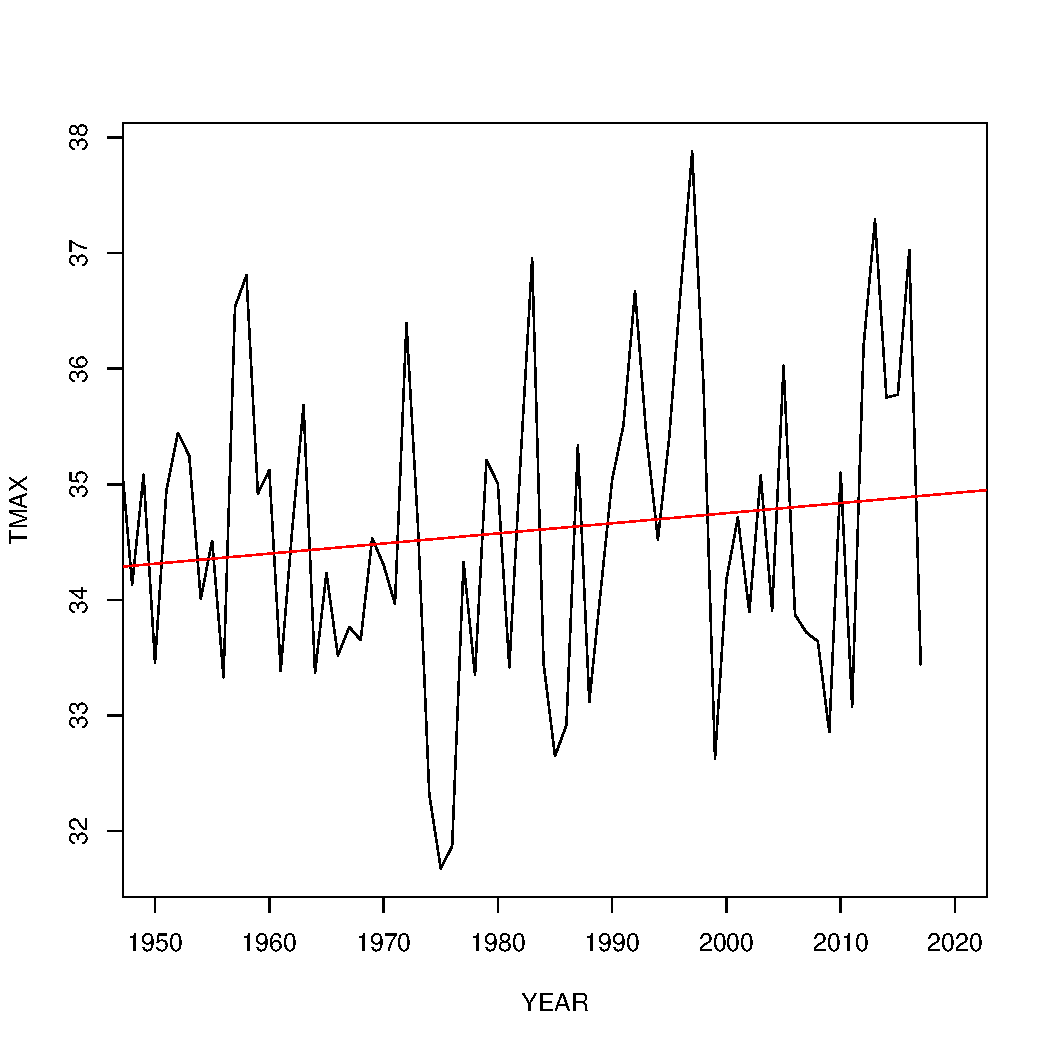
\includegraphics[width=\maxwidth]{figure/unnamed-chunk-5-1} 

\end{knitrout}
\caption{Some Caption.}
\label{fig:plotmissing}
\end{figure}

We find some rather odd low temperature values in the plot. We can find some of these with the \texttt{min()} function.

\begin{knitrout}
\definecolor{shadecolor}{rgb}{0.969, 0.969, 0.969}\color{fgcolor}\begin{kframe}
\begin{alltt}
\hlkwd{min}\hlstd{(climate_data}\hlopt{$}\hlstd{TMAX)}
\end{alltt}
\begin{verbatim}
## [1] -9999
\end{verbatim}
\end{kframe}
\end{knitrout}

\subsection{Re-assigning Missing Values to NAs}

What's going on?  What is the deal with the -9999? These are used for missing data. Historically, computers didn't have a lot of options for mixing numbers and letters in a variable type while R has some built in flexibility for this. So, to avoid leaving values blank (with all the ambiguous interpretations), the value -9999 is used to sybmolize missing values, since the number is unrealistic in the real world!

%Obviously, if we averaged the temperature with these values, we'd get a pretty inaccurate number (e.g. round(mean(climate\_data$TMAX), 0) versus round(mean(climate\_data$TMAX[climate\_data$TMAX>-9999]), 0). Thus, we need to remove them!  

We will replace the -9999 with NA, which R uses specifically to avoid accidently averaging arbitrary values that are representing missing values. 

How do we do this?
\begin{knitrout}
\definecolor{shadecolor}{rgb}{0.969, 0.969, 0.969}\color{fgcolor}\begin{kframe}
\begin{alltt}
\hlstd{climate_data}\hlopt{$}\hlstd{TMAX[climate_data}\hlopt{$}\hlstd{TMAX}\hlopt{==-}\hlnum{9999}\hlstd{]} \hlkwb{=} \hlnum{NA}
\hlstd{climate_data}\hlopt{$}\hlstd{TMIN[climate_data}\hlopt{$}\hlstd{TMIN}\hlopt{==-}\hlnum{9999}\hlstd{]} \hlkwb{=} \hlnum{NA}
\end{alltt}
\end{kframe}
\end{knitrout}


Okay, now we'll check again, but let's plot a just a few years, let's say five years (356 days * 5 years = 1825) or 1825 observations. 

\begin{knitrout}
\definecolor{shadecolor}{rgb}{0.969, 0.969, 0.969}\color{fgcolor}\begin{kframe}
\begin{alltt}
\hlkwd{plot}\hlstd{(TMAX}\hlopt{~}\hlstd{DATE, climate_data[}\hlnum{1}\hlopt{:}\hlnum{1835}\hlstd{,],} \hlkwc{ty}\hlstd{=}\hlstr{'l'}\hlstd{)}
\end{alltt}
\end{kframe}
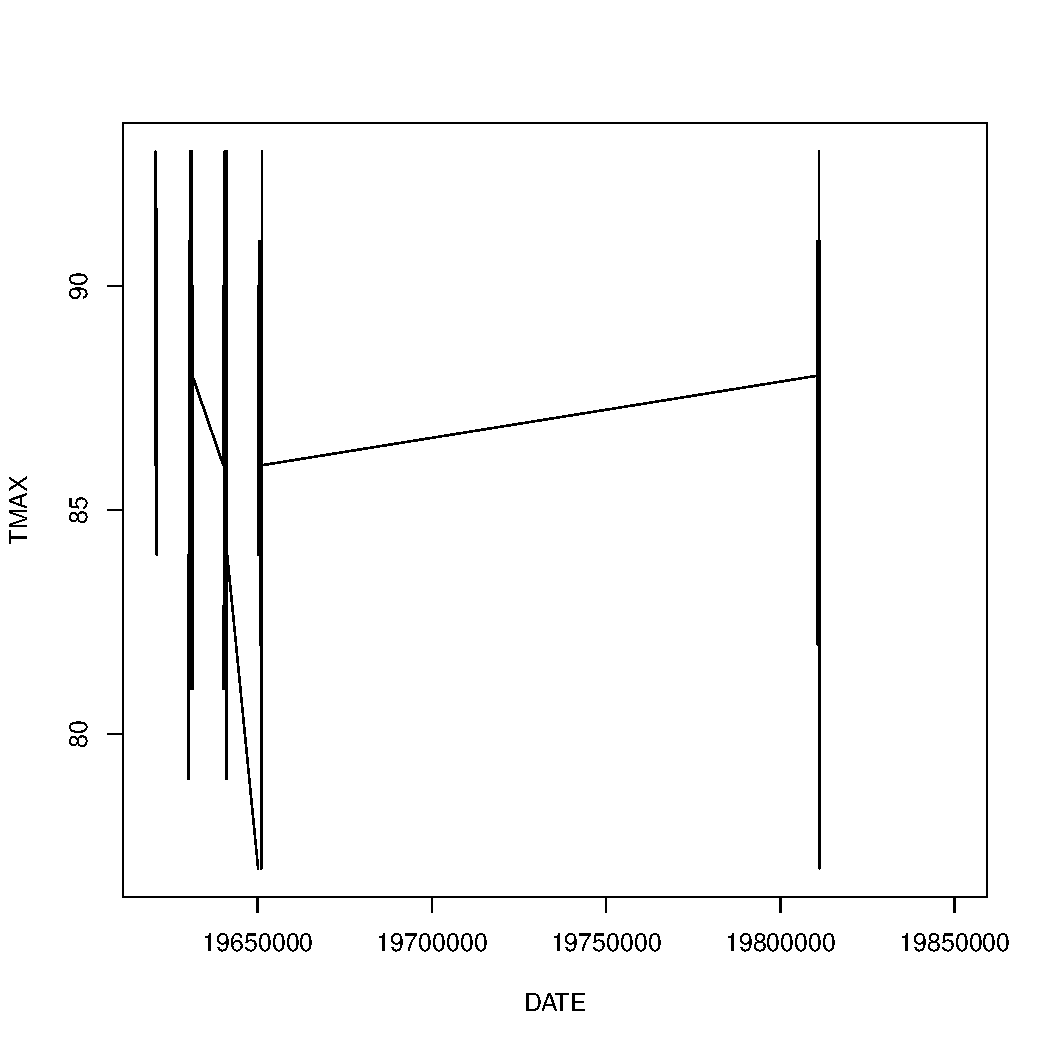
\includegraphics[width=\maxwidth]{figure/unnamed-chunk-8-1} 

\end{knitrout}

Yikes! What's wrong? It appears we have gaps in the data -- but we already removed our missing data, why are these big jumps in the data. 

As it turns out the problem is that with how the dates are specified. In particular, the Dec 31 to Jan 1 transition. Let's say that the data have a year change between 1913 and 1914. The date format in the NOAA data are YYYYMMDD, or year, month, and day with 4, 2, 2 digits, respectively. Thus, the last day of 1913 is 19131231 or Dec, 31, 1913. The next day is January 1st or 19140101. But when you plot these on the x-axis, the order of the values should be $19131231 \rightarrow 19131232 \rightarrow 19131233 \rightarrow 19131234$, etc but there is no 32nd, 33rd or 34th of December. Instead the dates go from  $19131231 \rightarrow 19140101$. We have lots of numbers that are skipped, but no coded as missing, but missing all the same. So, now we need to convert our dates to something more sensible. In R, that means creating a variable with a format that expects dates, thus doesn't plot numbers that are impossible dates!

\subsection{Converting Date Format}

To create a new format, we have to complete a few steps. Unfortunately, date formats are one of the more obtuse aspects of R, but if you follow along, you should have success, even if you have no clue what you did. 
First, we convert the date to a string of character values. Next, we'll convert the strings to a data format. 

\begin{knitrout}
\definecolor{shadecolor}{rgb}{0.969, 0.969, 0.969}\color{fgcolor}\begin{kframe}
\begin{alltt}
\hlstd{strDates} \hlkwb{<-} \hlkwd{as.character}\hlstd{(climate_data}\hlopt{$}\hlstd{DATE)}
\hlkwd{head}\hlstd{(strDates)}
\end{alltt}
\begin{verbatim}
## [1] "19620512" "19620516" "19620605" "19621006" "19621007" "19621012"
\end{verbatim}
\begin{alltt}
\hlstd{climate_data}\hlopt{$}\hlstd{NewDate} \hlkwb{<-} \hlkwd{as.Date}\hlstd{(strDates,} \hlstr{"%Y%m%d"}\hlstd{)}
\end{alltt}
\end{kframe}
\end{knitrout}

\subsection{Checking the New Dates}

\begin{knitrout}
\definecolor{shadecolor}{rgb}{0.969, 0.969, 0.969}\color{fgcolor}\begin{kframe}
\begin{alltt}
\hlkwd{plot}\hlstd{(TMAX}\hlopt{~}\hlstd{NewDate, climate_data[}\hlnum{1}\hlopt{:}\hlnum{1835}\hlstd{,],} \hlkwc{ty}\hlstd{=}\hlstr{'l'}\hlstd{)}
\end{alltt}
\end{kframe}
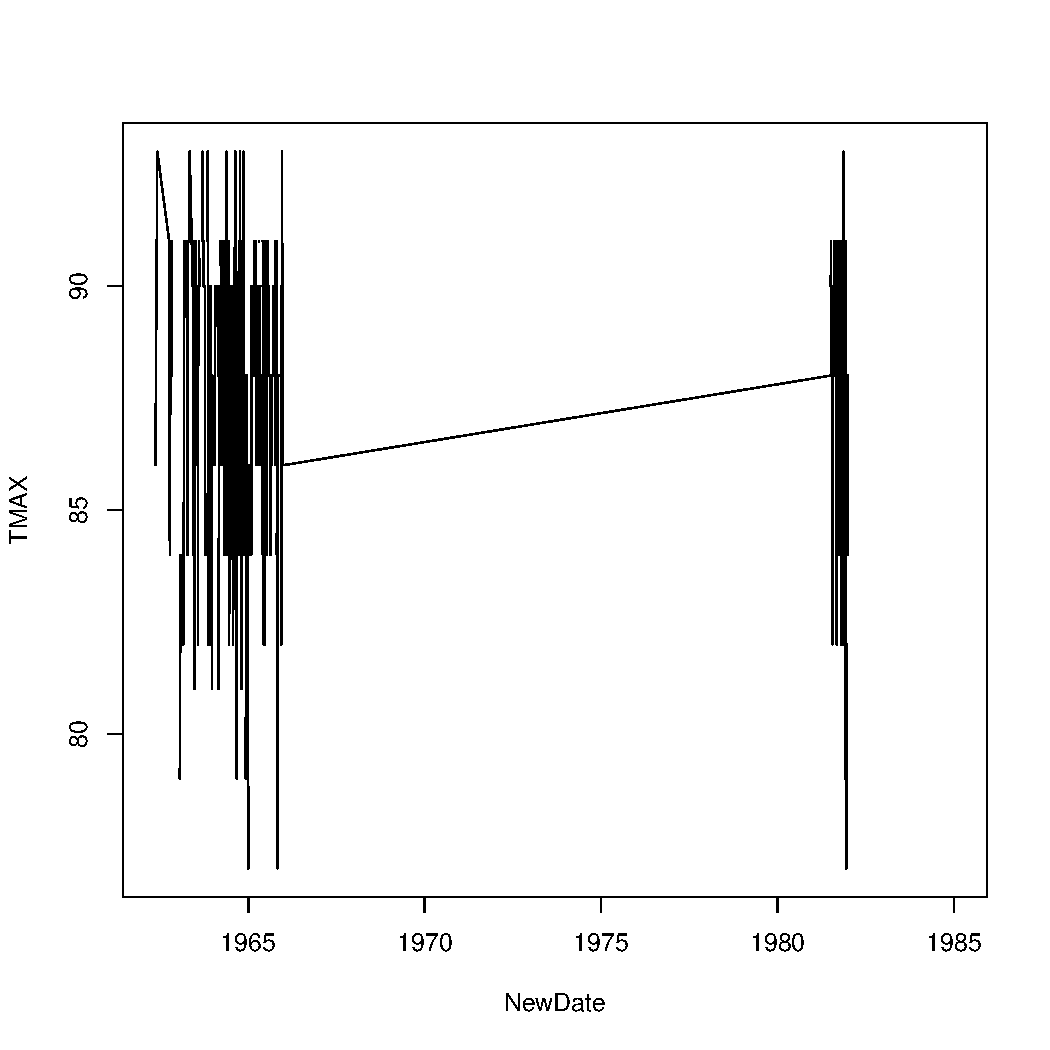
\includegraphics[width=\maxwidth]{figure/unnamed-chunk-10-1} 

\end{knitrout}

%\subsection{Subset Sites}

%unique(import$STATION_NAME)
%Let's choose the FAIRPLEX NY US because the record is longer than the airport.

%LosAngeles <- subset(import, STATION_NAME=="LOS ANGELES DOWNTOWN USC CA US", select=c(STATION, STATION_NAME, DATE, NewDate, TMIN, TMAX, PRCP))


%plot(TMAX~NewDate, LosAngeles, ty='l')





\begin{knitrout}
\definecolor{shadecolor}{rgb}{0.969, 0.969, 0.969}\color{fgcolor}\begin{kframe}
\begin{alltt}
\hlcom{#maunaloa$average}
\end{alltt}
\end{kframe}
\end{knitrout}

to dump the average CO$_2$ concentrations readings onto your screen as a vector. You should see some ~627 observations, depending on how recent the data have been uploaded. So, the dollar symbol is used to drill into the data frame vectors.  And when you look at the \texttt{str()} function again, you will see these dollar signs again.

\section{Preparing Records for Analysis}





\end{document}
